\documentclass[11pt,letterpaper]{article}

%\usepackage[latin1]{inputenc}
\usepackage[utf8]{inputenc}
\usepackage[cyr]{aeguill}
\usepackage[colorlinks=true]{hyperref}
\usepackage{textpos}
\usepackage{graphicx}
\usepackage[french]{babel}
\usepackage{color}
\usepackage{array}
\usepackage{enumerate}
\usepackage{fancyhdr}
\usepackage{lastpage}
\usepackage{amsmath}
\usepackage{amssymb}
\usepackage{epstopdf}
\usepackage{mathrsfs}
\usepackage{float}
\usepackage{caption}
\usepackage{subcaption}
\usepackage{siunitx}
\usepackage{minted}
\addto\captionsfrench{\def\tablename{Tableau}}

\usepackage[none]{hyphenat}
\usepackage[shortlabels]{enumitem}

%-----------------------------------------------------------------%
% Alias de commandes parce que les noms de
% commandes originaux sont pas intuitifs
\newcommand{\infini}{\infty}
\newcommand{\Ohms}{\Omega}
\newcommand{\e}[1]{\times 10^{ {#1} }}
\newcommand{\fleche}{\rightarrow}
\newcommand{\donc}{\Rightarrow}
\newcommand{\fois}{\times}
\newcommand{\environ}{\simeq}
\newcommand{\gras}{\textbf}
\newcommand{\italique}{\textit}
\newcommand{\boite}[1]{ \fbox{ \parbox{\textwidth}{#1} } }
\newcommand{\an}{\emph}
%-----------------------------------------------------------------%

%-----------------------------------------------------------------%
% Definitions
\newcommand{\session}{2023-2024}
\newcommand{\firstauthor}{Yann \textbf{Roberge}}
\newcommand{\firstregistrationnumber}{1802531}
%\newcommand{\secondauthor}{Yann \textbf{Roberge}}
%\newcommand{\secondregistrationnumber}{1802531}
%\newcommand{\reportnumber}{}
\newcommand{\firsttitle}{Revue de littérature}
%\newcommand{\secondtitle}{   }
%-----------------------------------------------------------------%


\oddsidemargin 0pt
\topmargin 0pt
\textwidth 6.5in
\textheight 8.1in

\setlength{\parskip}{1em}

\definecolor{bleu_poly}{RGB}{65,170,230}
\definecolor{vert_poly}{RGB}{140,200,60}
\definecolor{orange_poly}{RGB}{250,150,30}
\definecolor{rouge_poly}{RGB}{185,30,50}
\definecolor{gris_poly}{RGB}{166,168,171}


\title{\vspace{-2.5cm} \noindent\makebox[\linewidth]{\color{rouge_poly}{\rule{\textwidth}{1.5pt}}}
        \begin{center}
          \begin{tabular}{m{6cm}}
           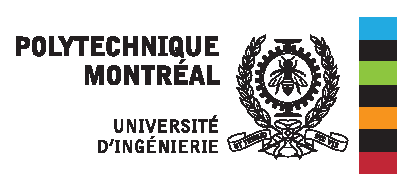
\includegraphics[width=0.4\textwidth]{Polytechnique_signature-CMYK-droite_FR.eps}
          \end{tabular}
        \end{center}
        \noindent\makebox[\linewidth]{\color{rouge_poly}{\rule{\textwidth}{1.5pt}}}
        \\ \  \\
        \Huge \firsttitle
        \\ \ \\
        }

\author{\session \\ École Polytechnique de Montréal}

\date{Dernière mise à jour: \today}

\pagestyle{fancy}

\lfoot{\session}
\cfoot{Chaire KIN}
\rfoot{\thepage/\pageref{LastPage}}
\chead{}
\lhead{\emph{Revue de littérature -- \firstauthor  \, (\firstregistrationnumber)}}
\rhead{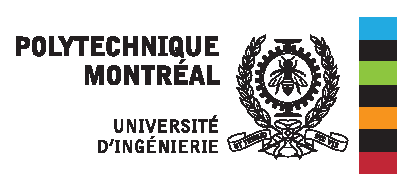
\includegraphics[width=2.5cm]{Polytechnique_signature-CMYK-droite_FR.eps}}
\renewcommand{\headrulewidth}{0.4pt}
\renewcommand{\footrulewidth}{0.4pt}
\setlength{\headheight}{45pt}


\graphicspath{{figures/}}


\newcommand{\vb}[1]{\mathbf{#1}}
\newcommand{\bs}[1]{\boldsymbol{#1}}


%-----------------------------------------------------------------%
% SOF
\begin{document}
\maketitle
\noindent\makebox[\linewidth]{\color{rouge_poly}{\rule{\textwidth}{1.5pt}}} 

\noindent \LARGE \firstauthor  \hfill \firstregistrationnumber

\noindent\makebox[\linewidth]{\color{rouge_poly}{\rule{\textwidth}{1.5pt}}}

\newpage
\normalsize


\section{Sujets par mots-clefs}

(Remplir plus tard quand il y aura ~75 références)

\clearpage

%%%%%%%%%%%%%%%%%%%%%%%%%%%%%%
\section{Résumés de lecture}

%%%% Résumés de lecture à la base écrits à la main, traduits et retapés ici

% Résumé de lecture

\subsection{P4: programming protocol-independent packet processors, \cite{bosshart_p4_2014}, Bosshart et al., 2014}
\gras{Pertinence:} 3 (article fondateur)
\gras{Sujets:} langage P4, SDN

\gras{Problématique:} Comment étendre les fonctionnalités des SDN sans rajouter une complexité hors de contrôle à Openflow?

\gras{Prérequis:} MPLS: \cite{noauthor_micronugget_nodate}, \cite{noauthor_multiprotocol_2023}; PortLand: \cite{noauthor_portland_2009}, \cite{noauthor_understanding_nodate}; VLANs, dot1Q: \cite{noauthor_vlan_2023}, \cite{noauthor_ieee_2022}; champ EtherType: \cite{noauthor_ethertype_2022}. Les trois sont utilisés à titre d'exemple. Openflow.


\gras{Réponse:} Arrêter d'ajouter toujours plus d'entêtes possibles à la spécification d'Openflow. Implémenter à la place un 'Openflow 2.0' qui soit indépendant du protocole, permette la reconfiguration du plan de données, et soit indépendant de la cible.

\gras{Résumé:} Les auteurs proposent le langage P4 comme Openflow 2.0. Le langage spécifié doit trouver un équilibre entre l'exhautivité de son support de protocoles et sa simplicité. Les développeurs P4 devraient pourvoir développer des modèles indépendant de la cible de la même manière que les développeurs C peuvent développer des programmes sans se soucier du jeu d'instructions`abstrait par le compilateur.

2 - Modèle abstrait

Les programmes suivront un modèle standard de commutateur formé d'une chaîne amorcée par un parseur (FSM), suivi d'une série de table \emph{match-action} et un désérialiseur (Le modèle qui allait devenir PISA.). Les auteurs font la distinction entre les opérations de \emph{configuration} et \emph{peuplement} (\emph{populating}, des tables), depuis renommées plan de données et plan de contrôle. Ils définissent les métadonnées comme information passée d'une table à une autre - port d'entrée, \emph{timestamp}, etc. L'AQM fonctionne commen sous Openflow: des tables d'actions distr5ibuent les paquets entre les ports de sortie; ils prévoient que l'on puisse ajouter d'autres fonctions de contrôle de congestion au langage.

3 - A programming language

Le P4 doit pouvoir définir le format de chaque entête. Des alternatives au P4 serient Click, et Openflow 1.0 lui-même. Le premier décrit le traitement de paquets avec une syntaxe C++ et vise l'implémentation de commatateurs logiciels. Il est difficile à synthétiser en matériel parce qu'il n'exprime pas le traitement sous forme de pipeline de flux de contrôle. Openflow 1.0 ne permet pas de définir librement des en-têtes.

4 - P4 by example

Ils utilisent l'exemple des étiquettes MPLS pour définir les structures et mot-clefs de base qui sont toujours dans le $P4_{16}$ aujourd'hui:
\begin{description}
	\item[Headers] champs d'entêtes, définition de leurs valeurs admissibles
	\item[Parsers] Machine d'identification d'entêtes (et de vérification)
	\item[Tables] Traitements à appliquer en fonction des entêtes \& actions
	\item[Controls] Blocs de contrôle de flux, menant d'une table à une autre.
\end{description}

Les tables interagissent avec le plan de contrôle SDN. Elles sont synthétisées sur les ressources de la cible: RAM pour les correspondances exactes (\emph{exact-match}), TCAM pour les correspondances ternaires (et pour les LPM je suppose?). La compilation est 'facile' pour des cibles logicielles, moins pour les ASICs. Le compilateur \emph{back-end} traduit la représentation parsée vers la cible matérielle.

\gras{Avis:} Le papier pose les bases du langage P4 et de la métaarchitecture PISA tels qu'on les connait aujourd'hui. À la base, l'objectif du langage était simplement de dépasser le manque de flexibilité intrinsèque des SDN; alors qu'aujourd'hui on met plus en avant les applications supplémentaires (INT, in-network computing, etc.) possibles sur les commutateurs P4. La syntaxe a beaucoup changé depuis 2014, surtout la FSM du parseur et les tables; mais toutes les idées de base se retrouvent déjà dans ce papier.
La possibilité de synthèse sur FPGA n'est pas même évoquée dans ce papier. Il faut croire que les choses ont changées depuis puisque je me souviens qu'à la keynote P4 de Mai 2022 M. McKeown affirmait que les commutateurs sont aujourd'hui plus rapides sur matériel reconfigurable que sur ASIC, parce que l'implémentation FPGA n'est pas obligée de s'encombrer de tout un tas de fonctionnalités niches dont la plupart ne seront jamais utilisées.

\clearpage

% Résumé de lecture

\subsection{Oracle VirtualBox User Manual, \cite{noauthor_oracle_2004}, Oracle, 2004-2023}
\gras{Pertinence:} 3 ; tous les environnements P4 et réseau en général passent par des VMs, donc autant savoir ce qu’on fait.
\gras{Sujets:} environnements de développements

\gras{Problématique:} Comprendre les réglages et les configurations réseaux possibles avec les VMs, dans le but d'arriver à monter facilement de nouveaux environnements.

\gras{Prérequis:} Aucun


\gras{Réponse:} Arrêter d'ajouter toujours plus d'entêtes possibles à la spécification d'Openflow. Implémenter à la place un 'Openflow 2.0' qui soit indépendant du protocole, permette la reconfiguration du plan de données, et soit indépendant de la cible.

\gras{Résumé:}

\begin{itemize}
	\item Section 4 : Configuring VMs. Ils passent à travers tous les réglages possibles du matériel. En particulier les réglages possibles des interfaces débogage sérielles. La plupart sont difficiles à utiliser parce que VBox n’a pas accès aux fichiers \texttt{/dev/ttyS*} de l’hôte.
	\item Section 7 : Virtual networking. Ils passent à travers tous les réglages des cartes réseau virtuelles : NAT, bridge, host NAT, internal network, d’autres accessibles hors du GUI.
\end{itemize}

On peut controller VBox entièrement par CLI avec VBoxManage. Certains fonctionnalités avancées ne sont accessibles que par ligne de commande, pas par le GUI.

Troubleshooting : s’ajouter soi-même au groupe UNIX \texttt{vboxusers}.

\gras{Avis:} En règle générale la configuration de VM se comprend très bien par analogie avec le montage de PC physique (insérer des cartes dans la carte mère), et les configuration réseau se comprennent comme des montages réseau avec des switchs et des routeurs physiques.

\clearpage

% Résumé de lecture

\subsection{P4 Network Programming Language—what is it all about?, \cite{parol_p4_2020}, Pawel, 2020}
\gras{Pertinence:} 3 (article d'introduction au P4)
\gras{Sujets:} langage P4

\gras{Problématique:} Quels nouvelles fonctionnalités réseau le P4 débloque-t-il? Quel est le potentiel d'usages du langage?

\gras{Prérequis:} Aucun

\gras{Réponse:} Décharger des couches de la pile réseau normalement gérées en CPU vers le NIC ou les commutateurs/routeurs: couche IP, TCP, NAT, pare-feu, etc. Simuler des designs de commutateurs; implémentation de nouveaux commutateurs logiciels. L'usage le plus prometeur est la possibilité de collecte de données de télémétrie directement sur les équipements réseau (\emph{in-band network telemetry}).

\gras{Résumé:} Le P4 a une structure de langage simple: il ressemble à du C allégé (ex. pas de pointeurs), auquel on a ajouté des mot-clefs natifs et des structures adaptées aux besoins des routeurs et commutateurs (entêtes, tables d'actions, déparseurs c-à-d sérialiseurs). Cela rend le p4 accessible aux ingénieurs réseaux n'ayant peu ou pas de d'expertise en semiconducteurs ou en logiciel. La facilité d'ajout de fonctionnalités leur donne la possibilité d'ajouter des fonctionnalités jusqu'alors hors d'atteinte, en particulier des mesures sur le réseau.

Les programmes P4 définissent le \gras{plan de données}, séquence de blocs faite d'un parseur d'entêtes suivi tables d'actions, du déparseur et d'autres blocs définis en-dehors du langage (\emph{externs}). Un P4 ne définit \emph{pas}, par contre, de quelle manière les tables sont remplies. Cette fonction est laissée au logiciel de contrôle SDN externe nommé \emph{plan de contrôle}. P4Runtime est l'un d'eux.

Le compilateur passe le programme vers une cible qui peut être n'importe quoi, d'un programme exécuté par un CPU, le commutateur simulé BMv2, du HDL pour un FPGA, ou des ASIC comme le Tofino. L'architecture P4 définit les contraintes de la cible, ce qui fait que les programmes P4 ne sont pas totalement portables.

\gras{Avis:} Un premier aperçu prosaïque de ce qu'est le P4 et ses applications commerciales les plus évidentes.

\clearpage

% Résumé de lecture

\subsection{What you should know about P4 programming language P4 programmable switch, \cite{noauthor_what_2022}, Afterfusion, Janvier 2022}
\gras{Pertinence:} 2 (article d'introduction au P4)
\gras{Sujets:} langage P4

\gras{Problématique:} Quel est l'intérêt du P4, et de quoi est fait un commutateur P4 physiquement?

\gras{Prérequis:} Aucun

\gras{Réponse:} Le P4 rend les commutateurs indépendants du protocole, permet aux ingénieurs réseau d'ajouter des applications maison dans leur équipement. Les commutateurs exécutent des fonctions du réseau normalement laissées aux OS des CPU: \emph{load-balancing}, sécurité, pare-feus, fonctions infonuagiques (je vois pas trop lesquelles), diagnostiques et télémétrie. Le Tofino possède pas mal le marché à lui tout seul.

\gras{Résumé:} On peut ajouter des features au ASIC après installation et l'adapter à n'importe quel protocole. Il y a déjà des exemples d'applications commerciales réussies: Facebook a un \emph{load-balancer} TCP sur le Tofino; Stratum vend des commutateurs intelligents avec fonctionnalité nuagiques dessus: \emph{load-balancer}, \emph{flow control}, INT. La télémétrie est difficile voire impossible à mettre en place avec des équipements traditionnels, parce qu'une télémétrie implémentée en logicielle ne peut pas être aussi rapide que le traffic commuté. Les auteurs en profitent pour faire la promotion de leur commutateur intelligent, qui intègre un Tofino, un x86 Intel et des SoCs ARM maison appelés DPU pour accélérer les fonctionnalités réseau comme la télémétrie.

\gras{Avis:} Un article commercial, mais qui a le mérite de montrer l'architecture d'un vrai matériel P4 fabriqué. Pour obtenir les features qu'ils voulaient, ils ont dû se rendre jusqu'à la fabrication d'un ASIC custom et payer la licence ARM dessus; ce qui montre bien que le Tofino est limité dans ce qu'il peut faire. Aussi, leur commutateur est un gros investissement monétaire... est-ce-que les fonctionnalité réseau supplémentaire justifient un tel prix.

\clearpage

% Résumé de lecture

\subsection{Getting started with P4, \cite{rijsman_getting_2019}, Rijsman, 2019}
\gras{Pertinence:} 3 (tutoriel pour monter une VM P4 et envoyer quelques paquets tests)
\gras{Sujets:} langage P4, environnements de développement

\gras{Problématique:} Quelles sont les étapes pour configurer un environnement P4 simple, monter un commutateur P4 basique, et le faire fonctionner sur le BMv2?

\gras{Prérequis:} Maîtrise de VirtualBox/VMWare/autre \cite{noauthor_oracle_2004} (l'auteur fait tout dans une boîte AWS, mais c'est quand même plus pratique avec une VM); protobuf; interfaces virtuelles Linux

\gras{Réponse:} Liste des étapes ci-dessous:

\gras{Résumé:}

\begin{itemize}
	\item Monter une VM Ubuntu 20.04.
	\item Ouvrir le SSH dessus (la manière la plus simple de le faire est de régler une IP statique sur la VM avec \texttt{netplan}, configurer le réseau de la VM en \emph{bridge}).
	\item Installer le million de dépendances \texttt{apt} - sauf \texttt{texlive-full}, je ne vois pas pourquoi ils suggèrent ce paquet plus lourd à lui seul que tout les autres, ça fonctionne très bien sans.
	\item Compiler et installer protobuf
	\item Compiler et installer BMv2
	\item Taper le code P4 basé sur \texttt{<core.p4>} et \texttt{<v1model.p4>}.
	\item Compiler avec \texttt{p4c} vers le BMv2. Ils sort un \texttt{.json} lisible par le simulateur comportemental.
	\item Ajouter une paire d'interface virtuelles \texttt{veth} à la boîte Linux.
	\item Lancer le commutateur \texttt{simple\_switch}, lui passer les interface virtuelles en option
	\item Lancer le plan de contrôle \texttt{simple\_switch\_CLI}, remplir la table de routage IP.
	\item Lancer des renifleurs de paquets sur les interfaces virtuelles, par exemple \texttt{tcpdump}.
	\item Envoyer des paquets test avec \texttt{scapy}. Selon l'IP de destination choisie ils apparaissent dans les fenêtres \texttt{tcpdump} en sortie.
\end{itemize}

\gras{Avis:} Le seul tutoriel de référence trouvable qui explique comment monter l'environnement de A à Z, sans utiliser la VM préfabriquée du répo officiel. Il marche du premier coup. Par contre il n'explique pas \emph{pourquoi} on a besoin de telle ou telle dépendance. Ça reste à explorer. Les outils sont déjà matures et fonctionne déjà bien. Reste à voir comment ça se passe quand on veut compiler vers des cibles matérielles.
\clearpage

% Résumé de lecture

\subsection{An exhaustive survey on P4 programmable data plane switches: taxonomy, applications, challenges, and future trends, \cite{kfoury_exhaustive_2021}, Kfoury et al., Mai 2021}
\gras{Pertinence:} 3 (excellente revue des domaines d'applications des commutateurs programmables). Les sections VI-XII pas analysées dans le détail.
\gras{Sujets:} télémétrie, \emph{load-balancing}, \emph{in-network computing}, \emph{middlebox functions}, IoT, sécurité, tests et vérification.

\gras{Problématique:} Quel est l'état de l'art des commutateurs à plan de données programmables, et dans quelles directions vont-ils continuer à évoluer?

\gras{Prérequis:} Aucun

\gras{Réponse:} Les équipements réseau numériques ont commencé dans un paradigme propriétaire, inflexible car de conception fermée. Le besoin d'interopérabilité et de standardisation a fait en sorte, dans ce paradigme, qu'il est extrêmement difficile de changer un protocole existant - la pile réseau s'\og ossifie \fg. Dans les quelques dernières années on a flexibilisé le plan de contrôle avec SDN, mais le plan de données est resté fixe. L'étape suivante naturelle a été l'émergeance de plan de données programmables, dont le P4 est devenu le langage standard de-facto. De nouvelles architectures de commutateurs en ont résultées. Les équipements propriétaires traditionnels vont être lentement mais surement remplacés par des équipements programmables.

\gras{Table des matières:}

\setlist[enumerate, 1]{label=\Roman*}
\begin{enumerate}
	\item Introduction
	\item Related surveys
	\item Traditional switches and SDN
	\item Programmable switches
	\item Methodology and taxonomy
	\item Surveyed work
	\setlist[enumerate, 2]{label=\Roman*}
	\begin{enumerate}
		\item In-band Network Telemetry
		\item Network performance
		\item Middlebox functions
		\item In-network computing
		\item IoT
		\item Cybersecurity and attacks
		\item Network and P4 Testing
	\end{enumerate}
	\item Challenges and future trends
	\setlist[enumerate, 2]{label=\Alph*}
	\begin{enumerate}
		\item Memory capacity (SRAM \& TCAM)
		\item Resource accessibility
		\item Arithmetic computations
		\item Network cooperation
		\item Control-plane intervention
		\item Security
		\item Interoperability
		\item Programming simplicity
		\item Deep programmability
		\item Modularity and virtualization
		\item Practical testing
	\end{enumerate}
	\item Conclusion
\end{enumerate}

\gras{Résumé:}

I - L'ossification des protocoles a eu lieu et est la conséquence directe du mainmise d'une poignée de fabricants d'équipement réseau sur le marché, utilisant des designs propriétaires non-reconfigurables. Le nombre de RFC sur les protocoles standards explose depuis les années 1990-2000, ce qui montre qu'il est difficile de faire changer un protocole pour soi sans forcer un changement au protocole sur tout le standard. Cela suggère qu'il faut changer de paradigme si l'on veut permettre à nouveau une innovation rapide sur les protocoles.

II - Jusqu'à ce jour il n'existait aucune revue exhaustive et extensive du langage P4. Les revues existantes ciblent des aspects spécifiques du domaine: Stubb sur les compilateurs et interpréteurs; Darghali sur la sécurité. Cordeiro sur les fonctionnalité et possibilités du langage. Satapathy sur l'évolution depuis les équipments fixes jusqu'à la SDN, puis au plan de données programmable. Bifulco sur la taxonomie des commutateurs programmables. Kaljic sur la SDN en général. Kamman sur la SDN aussi, mais en touchant aussi à la télémétrie et au \emph{in-network computing}. Tan sur l'évolution de la télémétrie pré-SDN, avec SDN, et avec le P4. Zhang sur le traitement \emph{stateful}.

III - La SDN permet aux opérateurs de diriger le plan de contrôle depuis un point central. Le P4 étend la SDN, la rend indépendante de la cible ([en principe!]). En règle générale, le cours naturel des technologies set d'évoluer du matériel et des langages fixes à des équipments programmables et programmés dans des langages haut-niveau. PISA est une architecture générique de cible pour le P4, de la même manière que le x86 est une architecture générale pour les CPUs programmés en C.

IV - PISA est le gabarit d'architecture d'un commutateur générique. Il définit le modèle général d'un parseur comme machine à état, suivi d'une chaîne de tables d'actions, elles-même composées de blocs de mémoires et de petits 'ALUs', le tout terminé par un sérialiseur programmable. Le $P4_{16}$ a étendu le $P4_{14}$ pour s'adapter à plus de cibles.

Avantages des commutateurs programmables: ils rendent l'adoption de nouvelles révisions plus rapide, renversent le flot de développement de \emph{bottom-up} à \emph{top-down}. Les opérateurs réseaux peuvent créer de nouvelles fonctionnalités pour obtenir un avantage compétitif sans avoir à le partager (ou le faire adopter dans un standard). Contrairement à ce à quoi on pourrait s'attendre, les équipements programmables améliorent la performance parce qu'ils peuvent ne contenir que les fonctionnalités dont on a besoin; là où les ASICs fixes doivent incorporer tout un tas de fonctionnalités secondaires, dont la grande majorité ne sera jamais utilisées, juste au cas-où.

L'écart de performances entre les puces de commutations et la commutation par CPU l'élargit de plus en plus: $\fois5-10$ en 1990-2000, $\fois 100$ maintenant. Cela s'explique par les multiples niveaux de parallélisme exploitables dans un ASIC/puce programmable: pipelinage entre l'\emph{ingress} et l'\emph{egress}, traitement de plusieurs entêtes en parallèle. En fait, le traitement parallèle de plusieurs champs en même temps fait que le commutateur se comporte comme un processeur VLIW, où l'entête du paquet est comme une longue instruction.

V - L'immense majorité (90 \%) des publications sur le P4 utilise soit des simulateurs comportementaux ([j'imagine BMv2]), soit des ASICs. Le 10\% restant fonctionne avec des smartNIC ou le NetFPGA.

Les sections VI-XII passent en revue toutes les applications possibles de la recherche dans le domaine.

VI - La INT est standardisée et spécifiée dans un document rédigé par Barefoot et d'autre entreprises du secteur. La INT donne beaucoup plus de visibilité sur le réseau que les outils du style \texttt{ping} et \texttt{traceroute}.

Fonctionnement standard de la télémétrie: un premier terminal étiqueté 'source INT' insère une entête 'instruction INT' n'importe où entre les entêtes existantes (pour ça reste flexible et indépendant du protocole). Celle-ci indique aux prochains routeurs traversés quelles mesures prendre. À chaque saut l'équipement ajoute une entête contenant les données récoltées d'après l'instruction. En bout de chaîne, le dernier saut enlève toutes les entêtes INT du packet et les poussent vers un noeud `INT collector' qui en fait l'aggrégation. Le reste du paquet est transmis à sa destination normalement, tout le processus de INT est transparent du point de vue de celle-ci.

La recherche actuelle en INT essaie de réduire son coût d'\emph{overhead} et de simplifier le traitement des données au collecteur.

VII - Les principaux problèmes de performance traîtés par la recherche P4 sont le contrôle de congestion et la gestion des file (AQM, Active Queue Management), les mesures de performance et les diagnostiques.

La plupart des mesures marchent avec des protocoles basées sur des requêtes, mais pour l'instant rien n'est standardisé/optimisé. La CC (contrôle de congestion) et la QoS (les deux sont liés) s'implémentent en séparant le traffic entre les équipements et en ralentissant le traffic à la source (\emph{throttling sender traffic}), le tout en exploitant les données de télémétrie et l'inspection jusqu'à la couche application.

VIII - Définition de \emph{middlebox}: équipement réseau utilisé pour réaliser n'importe quelle fonction autre que la commutation/routage classique, ex. NAT, conversion 4à6, 6à4, pare-feu.

Fonctions les plus étudiées en P4 : équilibrage des charges (demande du \emph{stateful processing}); les caches sur le réseau (\emph{in-network caches}) peuvent fonctionner mais demandent encore plus de travail: compression, choix des données à mettre en cache, minimisation de l'impact sur les performances globales; décharge de fonctions télécom (?), utiliser directement les commutateurs comme \emph{broker} de protocoles comme MQTT.

IX - Principaux candidats pour accélération-sur-réseau (\emph{in-network acceleration}): détermination du consensus dans les algorithmes par vote, phase d'aggrégation dans l'apprentissage machine. Pour le moment toutes ces pistes sont étudiées mais on ne fait tourner que des versions simplifiées des protocoles en question.

X - Les commutateurs intelligents peuvent aggréger les paquets de plusieurs appareils IoT en un seul avant de l'expédier. L'intérêt de l'aggrégation vient de la petite taille des données typiquement émises par ces appareils: les entêtes représentent une grosse part du coût des données. Le paquet aggrégé n'a qu'une seul entête et économise donc une partie des coûts. Mais ça se fait au prix qu'une latence allongée, puisqu'on attend que plusieurs paquets arrivent avant de les expédier.

XI - Les comm. int. peuvent agir sur la sécurité à toutes les couches du réseau.

Principaux usage: détection des \emph{heavy-hitters} (client utilisant une bande-passante trop large ou ayant un nombre anormalement élevé de connexions ouvertes) distribuée sur plusieurs commutateurs; sans télémétrie P4 on ne peut pas les détecter si leur traffic anormal est distribué entre plusieurs commutateurs/routeurs.

Autres fonctions de sécurité étudiées: implémentation de cryptographie sur le commutateur (pour le moment laissée aux terminaux), obfuscation de la topologie, cacher les entêtes de source/destination pour améliorer la vie privée; contremesures: détection DDoS, pare-feus à chaque couche (pas juste L3-L4), filtrage URL, filtrage de mot-clef.

XII - Les méthode de débogage réseau actuelles ne sont pas adaptées au matériel reconfigurable, qui offre beaucoup plus de services peu ou pas standardisés. Les possibilités ajoutées sont autant d'ouverture par les lesquels on introduit des bugs, susceptibles de perturber le réseau. Les travaux futurs pourraient travailler à ajouter de la résilience au réseau, en prévision : auto-diagnostics, auto-réparation à partir des données de télémétrie.

XIII - Défis et travaux futurs:

A - Limites sur la taille des mémoires: certaines applications, entre autres les caches-sur-réseau, font que l'on stocke de plus en plus de données dans de grandes tables.
$\Rightarrow$ Solution: utiliser des mémoires \emph{off-chip}, mais ça vient avec d'autre limites: bande passante, latence, etc.

B - Les implémentations P4 actuelles n'ont de mécanisme de bassin de ressources (\emph{pooling}), par exemple la mémoire des tables n'est pas partagée, et donc inefficacement utilisée.
$\Rightarrow$ Solution possible: avoir un bassin de mémoire centralisé et accessible depuis une Xbar? Idem avec des coeurs de processeurs.

C - Les calculs sur réseau sont limités par les contraintes de délais dans les nanosecondes, d'où la limite de leur complexité matérielle. Il n'est pas envisageable, par exemple, de faire du calcul à point flottant. Les applications implémentables sont donc limitées: difficile de faire de l'AQM, de la gestion de traffic, ou de l'apprentissage machine (qui implique généralement des points flottants).
$\Rightarrow$ Utiliser des approximations de fonctions avec pertes de précision, ou alors laisser le plan de contrôle précalculer des valeurs et stocker les résultats dans des tables.

D - Coopération sur la réseau: l'état du réseau doit être synchronisé entre les commutateurs, par exemple pour la gestion de traffic ou la détection DDoS
$\Rightarrow$ Il existe des protocoles comme P4Sync pour que les équipements puissent échanger des messages de contrôle entre eux.

E - Les interactions avec le plan de contrôle ralentissent le routage, ex. si un paquet ne correspond à aucune des entrées actuelles de la table. L'article ne suggère pas de solution concrêtes pour minimiser les appels au plan de contrôle.

F - En réponse à tous les problèmes de sécurité, les commutateurs devraient inspecter le traffic pour y repérer les patterns correspondant à des attaques.

G - Interopérabilité: les anciens équipements ne seront pas remplacés d'un coup par des équipements P4, il faut organiser la coexistence des deux pour un remplacement incrémental. L'une des possibilités sera de monter des commutateurs P4 par-dessus les lignes existentes pour écouter le traffic et collecter des données de télémétrie sans perturber le réseau existant.

H - La programmabilité a bien des avantages, mais ammène avec lui les difficultés intrinsèques du logiciel: les bogues inévitables et peuvent rester en production longtemps; la complexité mal gérée, l'élargissement de l'éventail de compétence demandées des opérateurs réseau.
$\Rightarrow$ Solution possible: des outils de développement plus visuels
$\Rightarrow$ Le compilation P4All et son extension de langage optimisent l'utilisation des ressources au lieu de la laisser aux programmeurs forcément imparfaits.

I - Dans un avenir plus ou moins lointain on peut envisager un réseau \og programmable en profondeur \fg, dans lequel tout les éléments du réseau (Serveurs, NICs, routeurs) sont programmables et capables de s'ajuster en fonction de la congestion du réseau en utilisant les données de télémétrie (système en boucle ouverte).

J - Reconfiguration à chaud: à l'heure actuelle les équipments sont mis hors-ligne pendant qu'ils sont reconfigurés ex. avec un nouveau programme P4. Il existe plusieurs frameworks implémentant la reconfiguration à chaud, mais tous ont un coût en performances.

K - La plupart des tests et vérifications sont faits en simulations/émulations de réseaux à petite échelle, parce qu'une simulation sur CPU ne peut pas atteindre le niveau de performances d'un réseau réel à grande échelle et à pleine charge. Il faut donc trouver un moyen de faire des tests physiques.
$\Rightarrow$ Solutions possible: TurboNet, un émulateur performant. P4Campus, une méthode pour chercheurs visant à tester une implémentation à l'échelle du réseau d'un campus universitaire.

L - L'opération du réseau par des humains se prête à l'erreur. Dans un futur distant on peut imaginer automatiser au complet le contrôle du réseau, avec un contrôle en boucle-fermée exploitant la télémétrie.

\gras{Avis:} Un tour d'horizon exhaustif et très bien écrit de toutes les possibilités des équipements programmables. C'est un point de départ utile pour trouver un sujet de recherche. Seul point manquant: l'aspect matériel n'est presque pas abordé; j'aurais aimé voir un commentaire sur les plateformes existantes en production et en prototypage.

\clearpage

% Résumé de lecture

\subsection{What you should know about P4 programming language P4 programmable switch, \cite{noauthor_reconfigurable_2022}, Wikipédia}
\gras{Pertinence:} 1 (source d'information générale qui n'a que but pour moi que de savoir que les FPGAs reconfigurables existent aujourd'hui commercialement.)
\gras{Sujets:} FPGA reconfigurable

\gras{Problématique:} Qu'est-ce-que le matériel reconfigurable, comment est-il implémenté sur le matériel, dans les grandes lignes?

\gras{Prérequis:} goulot d'étranglement de Von Neumann \cite{noauthor_von_nodate}: ralentissement de plus en plus problématique du bus entre le CPU et la mémoire principale.

\gras{Réponse:} Voir Résumé

\gras{Résumé:} Résumé: le moyen principal d’ajouter de la reconfigurabilité est d’avoir une architecture partiellement reconfigurable. Xilinx et Intel ont tous les deux certains modèles conçus pour être reconfigurables. Deux types de FPGAs partiellement reconfigurables:
Statique: on a pas besoin de réécrire tout le bitstream pour la reconfiguration, mais tout le FPGA doit être reset pendant le processus
Dynamique: plus intéressant, toute la partie non-reconfigurée du FPGA continue à fonctionner pendant qu’on reconfigure le reste.
La reconfigurabilité est permise par le design hiérarchique et modulaire: typiquement, on reconfigure une entité séparément du reste. Par exemple, un périphérique ou un coprocesseur connecté au CPU.

\gras{Avis:} Pas super, l’écriture part un peu dans tout les sens, passe trop de temps sur les différences entre FPGAs à granularité fine ou grossière. Pas de ligne directrice claire.

En 2008, quand Reconfigurable Computing \cite{hauck_introduction_2008} est sorti, il n'existait pas de puces commercialement disponible fait pour la reconfigurabilité (d'après ce même livre), parce que la taille du marché était alors trop petite. Je constate qu'il y en a maintenant quelques unes.

\clearpage

% Résumé de lecture

\subsection{Chapitre 1: Device Architecture, Reconfigurable Computing: The Theory and Practice of FPGA-Based Computation, \cite{chang_device_2008}, Chang, 2008}
\gras{Pertinence:} 3 (article de prérequis)
\gras{Sujets:} Architecture des FPGA

\gras{Problématique:} Qu'y a-t-il sous le capot d'un FPGA commercial classique?

\gras{Prérequis:} Aucun

\gras{Réponse:} (section 1.6: Sommaire) Les auteurs décrivent l'architecture d'un FPGA commerciale avec une approche \emph{bottom-up}: on décrit d'abord l'architecture des tuiles de base: LUT et DFF, regroupés en \emph{slices}. Ils décrivent ensuite l'interconnection des \emph{slices} en plus-proche-voisin à petit échelle qui les regroupe en CLB; puis, un niveau plus haut, comment les CLB sont interconnectés par le réseau de matrices d'interconnexions à plusieurs niveaux, dont les plus longs peuvent traverser plusieurs CLB de longueurs sont trop accumuler de délai de propagation. Des blocs spécialisés ajoutés au FPGA implémentent les opérations pour lesquelles les CLBs LUT/DFF sont inefficaces: RAM, DSP, PS. À chaque point d'interconnexion et chaque entrée de la table de vérité des LUT correspond un bit de configuration, stocké dans une mémoire SRAM, flash ou antifusible. Les modèles Xilinx Stratix et Altera Virtex illustrent comment ces structures sont utilisées en pratique.

\gras{Résumé:}

\begin{enumerate}
	\item{Logic - The computational fabric}
	\item{Arrays and interconnects}
	\item{Extending logic}
	\item{Configuration}
	\item{Case studies}
	\item{Summary}
\end{enumerate}

\gras{Logic - The computational fabric}

Blocs de base: les $n$-LUTs s'implémentent avec un mux à $n$ bits de sélection. Les $2^n$ bits d'entrée sont câblés à partir du bitstream à la configuration. Leurs choix déterminent la table de vérité de la fonction combinatoire implémentée.

Les plus grandes tables permettent des fonctions combinatoires complexes avec moins de délais de propagation que si elles étaient réparties entre plusieurs LUT, mais gaspillent des ressources si on implémentent des fonctions simples, ex. un inverseur 1-bit sur une LUT-6. Empiriquement, la LUT-4 est le meilleur compromis pour la plupart des applications.

En règle générale, les programmes de manipulation bit-à-bit bénéficient de LUT de granularité fine, tandis que les applications opérant sur des mots ex. DSP ou flux bénéficient de blocs grossiers. La solution standard est d'utiliser des LUT-4 épaulés par des blocs spécialisés en dur.

On rajoute un DFF optionnel à la sortie de chaque LUT pour pouvoir pipeliner ou implémenter de la logique séquentielle. Les \emph{CLBs} ont typiquement plus d'une LUT-4 pour optimiser le délai et la surface. Chaque entrée de chaque LUT, la valeur initiale de chaque DFF, et le mux pour sauter ou non le DFF, prennent chacun un bit dans la mémoire de configuration.

\gras{The array and interconnect}

Le interconnexions entre les \emph{slices} doivent pouvoir relier à peu près n'importe quelle tranche avec une autre, se croiser sans se perturber, et traverser de longues distances sans trop accumuler de délai.

Types d'interconnexions:

\begin{enumerate}
	\item{voisins-adjacents (\emph{nearest neighbor})}
	\item{segmentées}
	\item{hiérarchiques}
\end{enumerate}

Les FPGA commerciaux utilisent chacun leur variante d'interconnexions hiérarchiques: les tranches se rassemblent en petits groupes (\og îles \fg ou CLBs connectés uniquement à leurs voisins les plus proches; un mode d'interconnexion simple et direct, mais qui force tout signal propagé sur plus d'une case de longueur à traverser une tranche ou plus entre celle de départ et celle d'arrivée. Les tranches `transpercées' sont gaspillées, avec au passage un gros délai d'interconnexion.

Plusieurs îles se relient entre elles par connexions \emph{segmentées}; elles `nagent' au milieu des blocs d'interconnexions. Blocs rajoutés dans une interconnexion segmentées: \emph{Connection blocks} (CBs), qui relient ou pas les CLBs au bus d'interconnexion le plus proches (configurables), et \emph{Switch-Blocks} (SBs), crossbars placées aux croisement des bus horizontaux et verticaux, également configurables. Si on a besoin de fils plus longs que une case de CLB, les \emph{switch-blocks} peuvent commuter les fils sur des lignes sautant plusieurs (2, 4, 8...) cases sans passer par les commutateurs - et donc éviter les délais combinatoires associés. En règle générale, plus on monte dans la hiérarchie des groupes de logique de plus en plus gros, plus les SB offrent de long fils. Grâce à cette architecture, le délai de routage de A à B en fonction de la distance parcourue est $O(\log(n))$ et pas $O(n)$ comme on aurait pu s'y attendre. $\environ 90\%$ de la surface d'un FPGA est consacrée aux interconnexions!

\gras{Extending logic}

En plus des CLBs normaux, des tuiles supplémentaires accélèrent les opérations auxquelles la combinaison classique LUT-DFF est inadaptée, mais qui sont tout de mêmes courantes dans les applications: chaînes de retenues rapides pour les additionneurs, multiplieurs,, BRAMs, processeurs en dur. Au fur et à mesure que l'industrie applique les FPGAs à des domaines d'applications de plus en plus larges, on peut s'attendre à voir émerger un éventail de tuiles spécialisées de plus de en plus variées aussi.

\gras{Configuration}

Chaque point de configuration du FPGA correspond à un bit de mémoire. Le bitstream est stocké sur SRAM, Flash ou ROM antifusible.

Comparatif:

\begin{itemize}
	\item SRAM: rapide à écrire, pas d'usure, mais volatile (on doit rajouter une EEPROM externe), et consomme du courant statique
	\item Flash: Non-volatile, mais longue à écrire et sujette à l'usure.
	\item Antifusible: Invulnérable aux radiation (standard pour le spatial/militaire), mais OTP donc impossible à utiliser pour le prototypage ou les usages à FPGA dynamiquement reconfigurables.
\end{itemize}

Mémoires antifusibles: chaque bit a un lien ouvert par défaut, que se \og soude \fg quand on le programme.

\gras{Case studies}

L'Altera Stratix et le Xilinx Virtex (à jour à l'époque) utilisent les structures décrites dans les sections précédentes; avec chacun la nomenclature du fabricant: les éléments de bases sont essentiellement des LUT-4 avec un DFF - LE (\emph{Logic Element}) pour Altera, et tranche (\emph{slice}) pour Xilinx, nommées $X0Y0$, $X0Y1$, etc. en fonction de leur position dans l'île. Les regroupement (îles) d'éléments de base se ressemblent - LAB (Altera), CLB (Xilinx). Les deux ont plusieurs tailles de BRAM, des DSP, des chaînes de retenues rapides, et des processeurs en dur; le tout relié par des interconnexions hiérarchiques.

Les deux études de cas illustrent bien la pertinence et la - surprenante - précision des descriptions du matérielles faites dans ce chapitre.

\gras{Summary} (Avis ci-dessous)

\gras{Avis:} Un chapitre brillament écrit; par lequel un utilisateur passe d'un modèle mental du FPGA comme boîte noire \og soupe de portes logiques \fg cablées ensemble, à un modèle réaliste d'éléments logiques fixes, configurés par la mémoire du bitstream et routés à travers le réseau d'interconnexions hiérarchiques. Fort de cette conception, un designer peut baser ses designes HLS/RTL sur une compréhension solide du matériel et l'ajuster en fonction. Les auteurs le comparent avec justesse à un automobiliste qui ajuste sa conduite en fonction de sa compréhension de la mécanique du véhicule. Je verrais bien ce chapitre enseigné dans les dernières semaines d'un des cours d'introduction aux FPGA de 3\ieme année de bac élec.

\clearpage

% Résumé de lecture

\subsection{Getting Started with Alveo Data Center Accelerator Cards, \cite{amd_xilinx_inc_introduction_2022}, AMD Xilinx Inc., 2022}
\gras{Pertinence:} 1 (manuel d'installation des cartes Alveo, résumé succinct seulement)
\gras{Sujets:} Matériel

\gras{Problématique:} Comment installer les cartes Alveo, matériel \& configuration logicielle

\gras{Prérequis:} Aucun

\gras{Points saillants:} Les cartes sont fragiles; à manipuler avec un bracelet antistatique. Les versions sans ventirad monté sont faites pour être installées dans des serveurs déjà ventilés (on a les versions avec ventirad).

Setup logiciel: le logiciel de déploiement XRT est séparé de Vitis; avant d'utiliser la carte, utiliser les utilitaires fournis pour flasher plusieurs firmwares dans le carte, puis rouler le script de diagnostique pour vérifier l'installation. Détecter avec \texttt{lspci}.

Le chapitre 6 pointe vers l'ensemble de la documentation disponible pour la carte, utile pour la suite.

\clearpage

% Résumé de lecture

\subsection{Content-Addressable Memory (CAM) Circuits and Architectures: A Tutorial and Survey, \cite{pagiamtzis_content-addressable_2006}, Pagiamtzis K. and Sheikholeslami A., 2006}
\gras{Pertinence:} 3 (article de prérequis sur les mémoires CAM: les sections I et II donnent un background essentiel sur ce que sont les mémoires associatives, leurs architectures, et leurs circuits. Les sections III, IV et V, par contre, sont une revue de littérature passée-date sur les amélioration sur le CAM, plus niche et moins essentielles, pas nécéssaire de rentrer totalement dans les détails.)

\gras{Sujets:} Mémoires CAM

\gras{Problématique:} Comment implémenter une mémoire CAM en dur, au niveau système puis au niveau circuit? Comment réduire leur consommation de puissance?

\gras{Prérequis:} Fonctionnement du circuit d'une cellule SRAM \cite{noauthor_static_2023}

\gras{Réponse:} Au niveau système, une CAM prend en entrée une donnée et retourne l'adresse la contenant. Au niveau circuit, on l'implémente en CMOS avec une \emph{matchline} en logique NOR ou NAND, avec leurs variantes 9-T ou 10-T. La \emph{matchline} utilise un système de précharge, évaluation du résultat, puis amplification pour lecture du résultat. Les sections III, IV, et V, font l'inventaire des méthodes permettant d'économiser l'énergie en déviant des implémentations traditionnelles, au niveau de la \emph{matchline}, de la \emph{search line}, puis de l'architecture globale.

\gras{Résumé:}

I - Introduction: Les auteurs donnent un résumé du fonctionnement d'une CAM au niveau architectural. En règle générale la capacité des mémoires CAM suit la loi de Moore avec un retard de $\fois 2$ sur les SRAMs classiques; explicable par l'utilisation de 2 cellules SRAM pour chaque cellule de TCAM. 

A - Architecture générale d'une CAM: mot recherché en entrée, \emph{word-match} lines en sortie. Ces lignes de résultat de recherches passent un encodeur qui retourne l'adresse à laquelle on a trouvé le mot (encodeur de priorité dans le cas d'une TCAM, il faut stocker les préfixes les plus long dans les adresses basses.) (comment insère-t-on des ligne au milieu de la table alors? Il faut tout décaller?) Pour ensuite router le paquet vers le bon port de sortie, on enchaîne la CAM avec une RAM contenant la liste des ports de sortie. L'adresse sortie par la recherche en CAM rentre dans la RAM, qui retourne le port.

B - Bases des CAM: Ils rentrent un peu plus profond dans l'architecture. Chaque mot a une seule \emph{match line} (ML), partagée entre tout les bits du mot. Si un seul ou plus des bits de contenu ne contient pas le bit placé sur la \emph{search line} (SL), alors tout la ML se décharge (donc pas besoin de `porte ET' sur les bits). Les lignes préchargées passent au travers d'amplificateurs (\emph{Match-Line Sense Amplifier}, MLSA) avant de rentrer dans l'encodeur.

II - Core cells and Matchline structure: principaux circuits d'implémentation de cellules BCAM et TCAM.

\begin{description}
	\item[Cellules NOR 10-T:]{le classique. Une cellule SRAM flanquée de 4 transistors d'évaluation, deux de chaque côté du double-inverseur de la SRAM. Chaque paire de 2 transistors est reliée en série (logique ET), avec une grille sur la SL, et l'autre sur la BL (inversée par rapport à la SL). Si SL $\neq$ BL, alors la logique ET crée un chemin entre la ML et la masse et décharge la ML. On l'appelle NOR parce que la matchline n'est à `1' que si aucun des chemins de pulldown n'est activé.}
	\item[Cellules NAND 9-T:]{structure différente, avec moins de transistors mais dont la matchline accumule une perte de $V_{th}$ par bit, ce qui limite son intérêt. La chaîne de transistors le long de la matchline forme une porte `ET' (le MLSA inverse la sortie logique donc NAND).}
\end{description}

C - Cell variants: cellules moins courantes mais qui existent. 

\begin{description}
	\item[La NOR-9T:] qui fonctionnne sur le principe de la NAND-9T mais avec des chemins de pulldown. 
	\item[La NAND-10T:] qui fonctionne sur le principe de la NOR-9T, mais accumule aussi des pertes de seuils. Elle double même le nombre de seuils perdus puisqu'on a deux NMOS en série le long de chaque segment de la ML.
\end{description}

D - Ternary cells:

Il faut deux cellules SRAM-6T pour implémenter les trois états possible. Le dernier état en trop est interdit.

Encodage:
\begin{itemize}
	\item 0: $D = 0$
	\item 1: $D = 1$
	\item X: $D = 1$ et $\overline{D} = 1$ en même temps
\end{itemize}

Il y a deux manières de chercher avec des `don't care': 1 - stocker \texttt{`11'} sur la cellule, produit un \emph{match} peu importe la SL; 2 - Placer $SL = 0$ et $\overline{SL} = 0$ sur la \emph{searchline}, produit un \emph{match} peu importe les valeurs stockées dans les cellules.

On peut rendre le layout plus compact en remplaçant les NMOS par des PMOS, pour des raison d'agencement physique des transistors; mais ça vient avec la contrepartie de la faible mobilité des PMOS, qui ralentit la recherche et augmente la consommation d'énergie.

Il y a aussi des TCAM NAND, qui fonctionnent avec un bit masque (M) ajouté dans une cellule SRAM dédiée en parallèle au transistor \emph{match} d'une CAM NAND-9T normale: quand $M = 1$, la ML est toujours à 1 peu importe la BL (`X'). On peut aussi mettre $SL$ et $\overline{SL}$ à 0.

E - Structures de matchlines

NOR: La recherche se fait en 3 phases:
\begin{enumerate}
	\item Mettre les $SL$ et $\overline{SL}$ à 0 pour déconnecter les ML de la masse.
	\item Précharger les ML à `1' à travers un PMOS dédié à cette tâche.
	\item Charger le mot cherché sur les SL. Les résultats apparaissent en sortie du MLSA.
\end{enumerate}

La recherche NOR est rapide parce que la ML ne se décharge qu'à travers 2T dans le pire des cas (beaucoup moins que les NAND).

NAND: la ML est segmentée le long de la chaîne des BCAMs jusqu'au MLSA.
\begin{enumerate}
	\item Couper le transistor d'évaluation qui relie la chaîne de la ML à la masse.
	\item Charger les SL et $\overline{SL}$ avec le mot.
	\item Préchercher la \emph{matchline} à partir de son noeud le plus proche du MLSA. La tension se propage le long de la chaîne avec perte de seuils.
	\item Si tout les bits `trouvent' alors toute la ML est reliée à la masse par le transistor d'évaluation en bout de la ligne - $ML = 0$. Sinon, il suffit d'un seul transistor qui ne `trouve' pas pour couper la chaîne et faire en sorte que $ML = 1$ ($ML = 0 \donc \textrm{match}, ML = 1 \donc \textrm{non-match}$).
\end{enumerate}

Un problème de partage de charge se pose si la capacité du segement de ML préchargée est faible par rapport à celle l'ensemble de la ligne quand plusieurs transistors se ferment. La charge se diffuse le long de la ligne, donc la tension de précharge baisse. Elle peut baisser jusqu'au point où le MLSA détecte par erreur une tension basse - un faux \emph{match}. Pour y remédier on peut précharger les noeuds intermédiaires en mettent $SL$ et $\overline{SL}$ à `1', mais ça consomme de l'énergie.

Le gros avantage de la NAND est consommer peu d'énergie sur les cellules qui ne trouvent pas le mot, ce qui est le cas de la grande majorité des cellules, voire toutes sauf une, ne contiennent normalement pas le mot. L'énergie de précharge n'est pas dissipée dans la masse tant que la matchline n'est fermée sur tout les bits. Les NOR consomment au contraire quand on pas de \emph{match}.

Le plus gros défaut dans la NAND est son délai, qui augment avec le carré du nombre de bits par mot (R et C et série des transistors). On limite en général à 8 ou 16 bits en conséquence.

Les NOR-10T sont les plus utilisées en pratique.

III - Matchline Sensing Schemes

(à partir de ce point je ne fais que résumer les grandes idées)

\boite{\gras{Aparté:} Mémoire HBM $\fleche$ \emph{High-Bandwidth Memory}, type de dé de mémoire pour GPU placé dnas le même boîtier que celui-ci, relié au GPU par un \emph{silicon interposer}, pont entre les deux. Une HBM est un empilement d'un dé `contrôleur HBM' placé au bas de la pile en contact avec l'interposeur, et de plusieurs dés de DRAM par-dessus (3D \emph{stacked silicon}). Certains gros FPGAs Xilinx peuvent implémenter des CAM en HBMs \cite{noauthor_content_nodate}.}

A - Modèle de puissance de système de précharge conventionnel: les circuits de charge-décharge sont modélisés avec la capacité de la ML et la résistance des transistors de décharge. Ils en déduisent les équations de temps de lecture et de puissance. Pour synchroniser le timing de l'opération on peut ajouter un mot inutilisé mais qui décharge sa matchline sur chaque cycle et toujours sur le cas le plus long.

B - Low-swing: exemple d'une architecture qui précharge la ML a une tensions sous VDD avec un condensateur \emph{tank} de précharge, dont la charge vient s'étaler le long de la cpacité de la ML ensuite (moins d'énergie utilisée au total, sans qu'on aie eu besoin d'un rail de tension supplémentaire).

C - Current-race scheme: la ML et la SL se préchargent en même temps à VSS, donc les transistors de décharge se ferment ou pas. Ensuite, une source de courant tente de charger la ML à `1', à son rythme. Si un des bits était en échec, la ML reste à `0' car reliée à la masse (current-race avec la source de courant). Sinon, la ML charge un transistor jusqu'à $V_{th}$, et le résultat réécrit un latch.

D - Précharge sélective: évaluer les 2-3 premiers bits d'abord, n'évaluer le reste du mot que si les premiers bits trouvent. Implémentation: monter les premières cellules les plus proches du point de précharge en NAND, le reste en NOR. Les NAND ne transmettent la précharge aux autres cellules que si tous leurs transistors le long de la ligne sont fermés. Cette implémentation est un moyen simple et courant d'économiser l'énergie.

E - Pipelinage: la ML est subdivisée par des registres. La sortie de chaque registre sert de enable aux étages suivants; donc dès qu'un étage ne match pas la recherche cesse.

F - Current-saving: Idem que C, sauf qu'on ajout un contrôleur à la source de courant. Le contrôleur prend $V_ML$ en entrée, injecte d'autant plus de courant que $V_{ML}$ est grand; le résultat étant que $V_{ML}$ monte quand trouve, alors que l'on tire peu de courant si l'on rate (surtout si plusieurs bits ratent). L'approche économise donc beaucoup de courant.

Toutes les approches proposées économisent $\environ 1/3$ d'énergie par rapport à l'approche conventionnel, au prix d'une augmentation de complexité.

IV - Searchline Driving Approaches

En conventionnel on charge les SL avec des drivers faits d'une série d'inverseurs dont la taille augmente de façon exponentielle. Les approches dont la ML se précharge bas sauvent $50\%$ d'énergie sur la searchline, parce qu'on a pas besoin de décharger les SL pour éviter d'interférer avec la précharge ML ($50\%$ en moyenne des bits togglent par recherche).

Approche hiérarchique: les SL normales, partagées entre tout les mêmes bits d'un mot, sont renommées GSL (Global Search Line) et n'alimentent plus directement les cellules. À la place, les GSL se subdivisent en LSL dont chaque branchement individuel `nourrit' une cellule CAM. Si une ML d'un bit d'un mot se décharge (rate), alors on désactive les LSL de l'étage suivant, ce qui sauve de l'énergie (mais rajoute de la complexité, et les économies peuvent être annulées par l'empreinte de la circuiterie supplémentaire.)

V - Approches architecturales

1 - Subdiviser la mémoire en banques sélectrionnées (activées) par quelques-uns des bits du mot. Pose des problèmes de capacité quand une banque se remplit disproportionnellement par rapport aux autres.

2 - Précalcul: précalculer une valeur sur les contenus, ne cherche que dans les mots dont la valeurs précalculée correspond. Ex. calculer le nombre `1's, désactiver les mots qui ont un nombre différent (PB-CAM, \emph{Pre-Computation based CAM}), ce cas en particulier a l'avantage de permettre d'éliminer la moitié \og $\overline{SL}$ \fg des searchlines, par une coïncidence mathématique le résultat reste bon.

3 - Encodage alternatif: utiliser un encodage alternatif qui utilise l'état \texttt{11} normalement inutilisé des TCAM  pour augmenter la densité d'information. Chaque combinaison de 4 demi-cellules TCAM fait trouve sur jeu unique de chiffres parmi $\{0,1,2,3\}$. Les demi-cellules forment des groupes de 4 partageant la même ML locale (LML). On forme des mots plus longs en reliant plusieurs LML sur une même ML globale (GML). Cette approche énonomise de l'espace en CAM en regroupant plusieurs entrées d'une table exact-match, ternaire ou LPM en une.

VI - Future developments

Section obsolète puisque l'article date de 2006, mais ils prévoient du développement dans l'utilisation de nouveaux types de mémoires, en particulier non-volatiles: MRAM, FRAM, etc. 15 ans plus tard on dirait bien que ça ne s'est pas réalisé.

\gras{Avis:} Un excellent article d'introduction aux CAM, bien écrit, particulièrement dense en information. Les auteurs vont loin dans leur analyse des variations possibles sur le circuit de base des CAM. L'article ne fait cependant pas mention des émulation de CAM possible à partir de mémoire RAM; les utilisateurs FPGA devront creuser un peu plus.

\clearpage

% Résumé de lecture

\subsection{In-situ Programmable Switching using rP4: Towards Runtime Data Plane Programmability, \cite{feng_situ_2021}, Feng et al., Nov. 2021}
\gras{Pertinence:} 2
\gras{Sujets:} P4 reconfigurable dynamiquement, PISA

\gras{Problématique:} Comment reconfigurer des commutateurs programmables P4 sans interrompre le service (sans les éteindre/rallumer pendant la configuration)?

\gras{Prérequis:} ECMP \cite{noauthor_equal-cost_2023}, VRF \cite{noauthor_virtual_2021}

\gras{Réponse:} Le modèle PISA empêche la reconfigurabilité, parce que les différentes couches de protocoles sont couplées dans le même parseur, le même pipeline de contrôle et le même désérialiseur; ce qui fait que l'on ne peut pas retirer/ajouter une fonctionnalité sans chambouler l'ensemble du programme. Les auteurs inventent une nouvelle méta-architecture (IPSA) plus adaptée à la reconfigurabilité, proposent un nouveau compilateur adapté à celle-ci (rP4), et ajoutent un nouveau simulateur comportemental pour aller avec (\texttt{ipbm}). Leur architecture vient avec une pénalité de surface et d'énergie d'environ 15\%, après essai sur FPGA (sans pipelinage).

\gras{Résumé:}

I - Introduction et proposition de valeur

Les auteurs insistent sur la nécéssité d'ajouter la reprogrammabilité dynamique pour faires des tests de configurations, pouvoir installer puis retirer des fonctions de télémétrie INT dont on a besoin que temporairement, ajouter/enlever des fonctions de calcul-sur-réseau temporairement aussi, et expérimenter avec de nouveaux protocoles. La reconfigurabilité dynamique va aussi devenir essentielle au fur et à mesure qu'on avance vers des réseaux autonomes. Pour l'atteindre, ils réinventent toute la chaîne d'outils P4 depuis le début: méta-architecture, compilateur, simulateur.

II - L'architecture IPSA

Dans PISA, il y a un parseur, un pipeline de contrôle et un sérialiseur globaux pour toute la pile de protocole. L'implémentation de chaque couche réseau est fortement couplée aux autres; ce qui rend complexe toute mise-à-jour incrémentale. Leur architecture IPSA remédie à ce problème en séparant le traitement des couches, chacune placée dans un bloc dédié appelé TSP (Templated Stage Processor). Chaque TCP comprend le parseur, les tables et la logique de contrôle (pas de désérialiseurs). La pipeline d'un TSP à l'autre peut être flexible: les TSP peuvent être connectés linéairement, l'un après l'autre, ou un bus d'interconnexions (qu'ils appelent TM sans en définir l'acronyme) capable de sauter un ou plusieurs TSP; et qui connecte aussi le dernier TSP au désérialiseur global. Le TM permet d'insérer/enlever un TSP du pipeline sans reconfigurer toute la chaîne.

Concernant les tables, les TSP ne font que pointer vers des blocs de SRAM/TCAM allouée d'un bassin global auxquel les TSP sont connectés au moyen d'un crossbar.

III - Le rP4

Le rP4 est un nouveau langage basé sur P4 pour programmer selon le paradigme IPSA. Ils ont conçu toute une panoplie d'outils pour développer avec:
\begin{itemize}
	\item{\texttt{rp4fc} (rP4 front-compiler): transpile le P4 normal en syntaxe rP4, génère aussi l'API pour le plan de contrôle (?)}
	\item{\texttt{rp4bc} (back-compiler): donne un JSON adapté à la cible, qui indique sur quels blocs les TSP doivent être placés. Il peut aussi générer des m-à-j incrémentales, ajout/suppression de TSP dans le chemin. Leurs algorithmes priorisent la latence au détriment de la surface.}
\end{itemize}

IV - Implémentation et évaluation

Ils testent 3 cas, créés à partir d'une architecture de routage Ethernet/IP normale, avec une variation à chaque fois: C1) ajout de la fonction ECMP ; C2) ajout du SRv6 ; C3) insertion d'un renifleur de paquets. Ils codent eux-même une implémentation VHDL de PISA, puis de IPSA (ce qui fait que leur comparaison est plus ou moins biaisée mais passons). Ils programment aussi leur compilateur et un utilitaire en ligne de commandes pour charger/décharger les modules.

Résultats: Au final les bandes-passantes sont divisées par trois avec IPSA; mais c'est surtout parce qu'ils ont pas encore pipeliné leur implémentation pour atteindre les une instruction par cycle. Les temps de compilation/flashage des mises-à-jour incrémentales sont divisés par 5-10 par rapport à une recompilation/reconfiguration intégrales PISA. De même pour la compilation et mise-à-jour de modèles comportementaux avec leur simulateur \texttt{ipbm} par rapport à \texttt{bmv2}.

V - Synthèse matérielle et résultats

Ils implémentent leur modèle sur Alveo 280. Leur implémentation prend \~15\% plus de LUT, 60\% plus de DFF (!), même si les DFF sont pas si important que ça.

La consommation d'énergie est supérieure à partir de 5 TSP, c'est-à-dire pour toute implémentation réaliste, mais les auteurs considèrent que pour un design avec énormément d'étages IPSA devrait diminuer la consommation totale puisqu'il permet d'éteindre les coeurs non-utilisés.

VI - Littérature similaire

D'autres solutions visent le même but que la leur, mais avec des limites: parfois la solution incrémentale n'est pas transposable en matériel, parfois ils faut quand même recompiler tout le programme pour une màj incrémentale.

\gras{Avis:} Un framework très intéressant; j'aime beaucoup leur idée de réduire le couplage entre les étages dans le parseur et le contrôle. Leur méthode de màj incrémentale me parrait aussi très utilisable. Ils ont tout implémenté sur FPGA; il serait intéressant de voir comment on peut partitionner leur architecture sur un système hétérogène.

\clearpage

% Résumé de lecture

\subsection{Bridging the Gap: FPGAs as programmable switches, \cite{luinaud_bridging_2020}, Thomas Luinaud, Thibaut Stimpfling, Jeferson, Pr. Savaria, Pr. Langlois, 2020}
\gras{Pertinence:} 2 (article de contribution, poussé la compréhension au fond quand même)
\gras{Sujets:} P4->HDL

\gras{Problématique:} Quels sont les goulots d'étranglement qui limitent l'utilisation des FPGA dans les commutateurs P4? Comment y remédier?

\gras{Prérequis:} Architecture des FPGA: \cite{chang_device_2008}

\gras{Réponse:} TODO

\gras{Résumé:} TODO

\gras{Avis:} TODO

\clearpage


% Thèses ''Trois mousquetaires''
% Résumé de lecture

\subsection{Fully Programming the Data Plane: A Hardware/Software Approach, \cite{santiago_da_silva_fully_2020}, Jeferson Santiago Da Silva, 2020}
\gras{Pertinence:} 3 (sa thèse, en plein dans le sujet)
\gras{Sujets:} P4->HDL

\gras{Problématique:} TODO

\gras{Prérequis:} Aucun

\gras{Réponse:} TODO

\gras{Résumé:} TODO

\gras{Avis:} TODO

\clearpage

% Résumé de lecture

\subsection{Algorithmes et architectures pour l'implémentation de la détection d'expressions régulières, \cite{luinaud_algorithmes_2017}, Thomas Luinaud, 2017}
\gras{Pertinence:} 2 (sa thèse)
\gras{Sujets:} Sécurité, Inpection profonde de paquets

\gras{Problématique:} TODO

\gras{Prérequis:} Aucun

\gras{Réponse:} TODO

\gras{Résumé:} TODO

\gras{Avis:} TODO

\clearpage

% Résumé de lecture

\subsection{Mémoires Associatives Algorithmiques pour l'Opération de Recherche du Plus Long Préfixe sur FPGA, \cite{stimpfling_memoires_2020}, Thibaut Stimpfling, 2020}
\gras{Pertinence:} 3 (sa thèse)
\gras{Sujets:} P4->HDL, recherche LPM

\gras{Problématique:} Comment accélérer la recherche LPM sur FPGA? Comment pourrait-on spécialiser les FPGA pour les applications réseau?

\gras{Prérequis:} 

\gras{Réponse:} TODO

\gras{Résumé:} TODO

\gras{Avis:} TODO

\clearpage


% Soumission P4 Workshop 2023
% Résumé de lecture

\subsection{DR-PIFO: A Dynamic Ranking Packet Scheduler Using a Push-In-First-Out Queue, \cite{elbediwy_dr-pifo_nodate}, Mostafa Elbediwy et al., Mars 2023}
\gras{Pertinence:} 1 (juste pour reste à date sur ce que fait le groupe)
\gras{Sujets:} gestionnaires de traffic

\gras{Problématique:} Comment tester les gestionnaires de traffic P4?

\gras{Prérequis:} Aucun

\gras{Réponse:} 

\gras{Résumé:} 

I - Introduction

\gras{Avis:} 

\clearpage


% Résumé de lecture

\subsection{One for All, All for One: A Heterogeneous Data Plane for Flexible P4 Processing, \cite{santiago_da_silva_one_2018}, Jeferson Santiago da Silva, 2018}
\gras{Pertinence:} 3 (un des rares papiers sur les plans de données programmables, en plus c'est de notre groupe)
\gras{Sujets:} Plans de données hétérogènes

\gras{Problématique:} Comment combiner les points forts de plusieurs cibles P4?

\gras{Prérequis:} Aucun

\gras{Réponse:} Ils créent le concept de HDP, plan de données hétérogène, plateforme comprenant plusieurs cibles en une.

\gras{Résumé:} 

I - Introduction

Les cibles P4 sont soit flexibles mais lentes (CPU, FPGA), soit performantes mais rigides (ASIC). Les externs de l'un ne sont pas transférables à l'autres. L'idée du papier est d'intégrer plusieurs cibles en parallèle sur le chemin de données, par exemple un FPGA utilisé avec un ASIC. Le FPGA n'est pas utilisé que comme accélérateur d'une cible mais bien comme cible à part entière.

II - Plan de données hétérogènes

Un programme P4 générique serait compilé par un outil dédié vers plusieurs cibles. Il n'est pas fait mention du partitionnement explicitement. La communication entre les plusieurs cartes peut se faire par Ethernet ou PCIe.

III - Preuve de concepts

 Ils ont pas encore implémenté le compilateur/partitionneur, leur test s'est fait avec un partitionnement à la main, BMv2 (à ce moment-là il y avait pas la switch Tofino au lab) + FPGA ZCU706, P4 compilé sous SDNet. En guise de résultats ils ont implémenté une switch L2, et vérifié qu'ils arrivaient à la partitionner, utiliser des externs agnostiques (?), et étendre les tables sur la DDR3 de la carte FPGA sans affecter les performances.

\gras{Avis:} L'intérêt de l'article est d'introduire l'idée de plateforme hétérogène, qui n'existait pas jusqu'alors, et ouvre beaucoup de portes. L'article est court, et n'a pas encore de résultats quantitatifs. Un bon point de départ pour nos travaux sur le HDP. Si ça en avait tenu à moi je l'aurais appelé \emph{plan de données composite}, pas hétérogène.

\clearpage

% Résumé de lecture

\subsection{Flightplan: Dataplane Disaggregation and Placement for P4 Programs, \cite{sultana_flightplan_2021}, Sultana, 2021}
\gras{Pertinence:} 3 (article d'introduction à l'outil le plus abouti pour l'hétérogène)
\gras{Sujets:} Plans de données hétérogènes

\gras{Problématique:} Comment rendre le code P4 réellement indépendant de la cible, et supporter les plans de données hétérogènes?

\gras{Prérequis:} Plans de données hétérogènes \cite{santiago_da_silva_one_2018}

\gras{Réponse:} Leur outils FlightPlan, qui partitionne automatiquement les sections d'un code P4 générique, puis le transpile vers un P4 spécifique à chaque cible et compilable avec les outils pré-existants. L'outils prend en entrée, entre autres, les définitions des cibles, la topologie du plan de données et les priorités (latence/débit/surface/énergie) du système.

\gras{Résumé:} 

Plan:

I - Importance de la désaggrégation

À l'heure actuelle, les compilateurs P4 ne prennent qu'une cible à la fois. Le programmeur ne peut donc pas faire abstraction du matériel par rapport au programme; et certains programmes ne peuvent pas tourner sur des cibles rapides mais inflexibles (ex. Tofino) ou flexibles mais trop lentes (CPU). La désaggrégation résoud ces deux problèmes en créant un niveau d'abstraction au-dessus du P4 spécifique au matériel et en combinant les meilleurs caractérisques de plusieurs cibles, et en évitant les pires.

II - Difficultés d'implémentation des plans de donnée hétérogènes

La désaggrégation manuelle serait trop difficile parce qu'il faudrait connaître tout le détail des besoins de l'application et ceux du matériel. C'est le genre de complexité qui peut être soulagée par des outils.

III - Description de leur solution

Flightplan prend en entrée un programme P4 agnostique au matériel, et retourne plusieurs programmes P4 spécifiques aux cibles. Son fonctionnement se fait en trois phases:

\begin{itemize}
	\item Analyse: sépare le code en segments, estime ses besoins en ressources
	\item Génération de `plan': assigne les segments aux cibles, les fusionne si ça permet d'optimiser.
	\item Gestion des programmes en cours de fonctionnement
\end{itemize}

L'analyseur génère des règles en fonction du code P4 monolithique, une description des cibles, la topologie et d'autres choses dont les priorités du système. Le résultat donne des programmes P4 passés aux compilateurs existants ex. SDNet ou p4c vers le BMv2.

IV - Évaluation

Leurs résultats montrernt que les HDP peuvent rajouter ou enlever de la latence, selon les cas. L'ajout de latence vient du traffic échangé entre les cibles pendant le traitement, et de l'ajout de métadonnées en plus (?).

Ils ont un utilitaire en ligne de commande pour contrôler l'exécution du programme.

\gras{Handover} (définition vocabulaire): émission d'un paquet d'une cible vers une autre au sein même du plan de donnée.

L'auteur a publié une vidéo pour la conférence NSDI2021, mais qui ne donne pas d'information en plus par rapport au texte.

\gras{Avis:} Le billet de blog est un résumé de leur article détaillé sur le fonctionnement de FlightPlan. Ils l'ont testé sur un banc de test matériel de taille impressionante: Tofinos, 5-10 cartes FPGA, le tout fait la taille d'une armoire. Cependant, les fichiers de configuration ex. propriété des cibles, etc. sont complexes, une mise en oeuvre pratique va probablement s'avérer très complexe et impliquer d'appeler les auteurs. Aussi, Flightplan ne segmente pas automatiquement le programme: le programmeur doit lui-même annoter les blocs de code pour définir les segments à partitionner.

Ils ont aussi une démo avec une figure en 3D qui illustre la circulation des paquets sur le plan de données désaggrégé; sensée donner un visuel intuitif de la topologie, mais je ne la trouve ni claire ni intruitive.

\clearpage


% Résumé de lecture

\subsection{The P4$\rightarrow$NetFPGA Workflow for line-rate packet processing, \cite{ibanez_p4_2019}, Ibanez, Brebner, McKeown, Zilberman, Fév. 2019}
\gras{Pertinence:} 2
\gras{Sujets:} P4->HDL, Outils

\gras{Problématique:} Comment compiler directement le P4 pour un FPGA, sans passer par l'étape de codage HDL?

\gras{Prérequis:} (Optionnel) SNMP \cite{noauthor_simple_2023} \cite{digitalocean_introduction_nodate}

\gras{Réponse:} Leur plateforme NetFPGA, s'appuie sur le compilateur Xilinx SDNet. Le HDL produit par SDNet cible le modèle de commutateur simple SimpleSUMESwitch, conçu d'abord pour l'enseignement.

\gras{Résumé:} 

I - Introduction

Les versions précédentes de la NetFPGA devaient se programmer en HDL; maintenant ils proposent un flot de conception pour obtenir des designs fonctionnels en écrivant que du P4. Étant donnée que toute l'industie s'est standardisée sur P4, il faut que les cibles se standardisent dessus aussi.

II - La langage P4 en général

Rappels sur ce que sont un parseur P4 et un bloc de contrôle. Rappels sur la syntaxe du parseur des états, extractions d'en-têtes, blocs de contrôle, logique \texttt{apply}, actions, tables. Idem pour les bus de métadonnées. Idem pour les \texttt{extern}.

III - SDNet

Xilinx avait créé SDNet à la base pour son propre langage PX, similaire mais antécédant à P4. Avant 2019 il transpilait le P4 en PX, et depuis il compile directement le P4. Il en sort des modules Verilog (SystemVerilog sur la dernière version?), et un banc de test SystemVerilog, un pilote C pour le plan de contrôle et un modèle C++ (pourquoi faire?). Le résultats prend $\environ2\fois$ plus de ressources qu'un modèle VHDL fait à la main (!).

IV - La carte NetFPGA SUME 10G

Les NetFPGA existante depuis 15 ans. Les commutateurs implémentés dessus utilisent l'architecture suivante:

$$ MAC (SFP ou DMA Rx (?)) \fleche Input arbiter \fleche Output port lookup (le P4 compilé vient dans ce bloc) \fleche Output queue (BRAM) \fleche MAC (SFP ou DMA Tx (?))$$

Le tout est contrôlé par un $\mu$Blaze connecté par AXI.

V - Le flot P4$\rightarrow$NetFPGA

On devrait pas avoir à toucher au code HDL, juste au P4, pour obtenir un commutateur fonctionnel. Les \texttt{externs} servent surtout à implémenter tout ce qui est \emph{stateful} - d'ailleurs ils en ont un certain nombre de déjà implémentées et utilisables pour ça. On peut ajouter nos propres externs, implémentés en HDL. Il faut ensuite les ajouter à des fichiers de configurations (lesquels?).

Les simulations se font en deux étapes
\begin{enumerate}
	\item Lancer le testbench généré par SDNet avec des paquets générés.
	\item Rouler une commande qui intègre le HDL SDNet sortant au NetFPGA, et le simuler.
\end{enumerate}

L'outil génère aussi une API Python pour le plan de contrôle; pour être précis c'est un wrapper par-dessus les API C générées par SDNet.

Le flot de conception ne supporte que le SimpleSumeSwitch. Pour d'autres architectures, il faut remettre les mains dans le HDL.

VI - Cas d'utilisation en recherche en enseignement

Beaucoup de travaux de recherche ont déjà été implémentées avec P4$\fleche$NetFPGA: télémétrie, \emph{load-balancer}, etc.

VII - Améliorations futures

Ils veut intégrer P4Runtime à la chaîne d'outils à la place de l'API Python existante, et rendre l'arhcitecture plus flexible dans la NetFPGA elle-même pour qu'on soit plus limités à l'architecture SimpleSumeSwitch.

VIII - Comparaisons aux solution P4-à-HDL existantes

Il y a eu beaucoup de tentativves de faire de la compilation P4 par l'intermédiaire de HDL: C, C++, Bluespec. Celui de Benacek \og P4-to-HDL \fg est en source fermée donc pas utilisable par la communauté.

IX - Comment commencer à l'utiliser: suivre les tutoriels en ligne pour faire fonctionner la chaîne d'outils. Ils espèrent avoir des contributions.

X - Conclusion: La NetFPGA remplit bien son rôle d'intermédiaire entre l'émulation logicielle et les ASICs très chers.

\gras{Avis:} Les auteurs comparent leur solution aux flots P4->HLS->FPGA existants (ils citent Jeferson \cite{santiago_da_silva_p4-compatible_2018}). Leur solution se démarque par sa facilité d'utilisation: elle est intégrée aux outils et passe directement du P4 au FPGA sans passer par l'intermédiaire d'un HLS, et maintenue sur le long terme (on le saura!)

\boite{
\gras{Aparté:} Le SNMP (\emph{Le Simple Network Management Protocol}. Un outil standard de gestion de réseau. Il est utilisé pour créer des outils plus haut-niveau. Un \emph{manager} gère un ensemble d'agents SNMP, à travers un jeu de (7) commandes de base. Les agents sont adressés avec une notation en décimal pointé (MIB, \emph{Management Information Base}). Ça s'installe relativement facilement sur des serveurs \cite{digitalocean_how_nodate}.

}

\clearpage


% Intel expandable architecture: leur produit hétérogène avec Tofino + FPGA
% Résumé de lecture

\subsection{Baidu Intelligent Cloud - Intel® Tofino™ Expandable Architecture, 2022 (je pense)}
\gras{Pertinence:} 2 (un cas pratique de l'utilisation de l'hétérogène)
\gras{Sujets:} HDP

\gras{Problématique:} Comment intégrer un plan de données hétérogène avec Tofino dans une application commerciale?

\gras{Prérequis:} Aucun

\gras{Réponse:} 

\gras{Résumé:} Les auteurs se servent du Tofino comme \emph{Cloud Gateway} entre l'intérieur et l'extérieur du centre de données. Avant ils utilisaient des commutateurs traditionnels, qu'ils ont remplacés par des x86, puis par des Tofinos. Leur prochaine étape est le système hétérogène Tofino/FPGA pour augmenter la taille des tables.

\gras{Evolving Cloud Compute and Memory Architectures}

Les charges de travail du nuage moderne ont des besoins en ressources de plus en plus variés et déséquilibrés (ex. mémoire, CPU, GPU, accélérateurs). Pour les gérer on a déjà les VMs et les conteneurs, qui séparent les environnements et regroupent les ressources en CPU/Mémoires. La désaggrégagtion des cibles est le prochain pas naturel de la virtualisation.

\gras{Evolving Cloud Network Architectures and Gateway}

Ils sont intéressés par le P4 et le Tofino pour le calcul-sur-réseau, la télémétrue et l'accélération ML. Au fur et à mesure que les charges augmentent on peut plus jsute rajouter des Tofinos horizontalement; on manque de place pour les tables: $\environ $ 1M entrées pour le VxLAN et le VM-NC, 100M pour le SNAT, des dizaines de Go pour les buffers de sortie. Les cartes FPGA sont utilisées pour leurs mémoires.

\gras{Usage du Tofino avant l'hétérogène}

Ils servaient de routeurs virtuels pour des sous-réseau virtuels de VMs et VPCs. Ils mettent aussi des filtres de paquets, pare-feu, et autres.

Usage principal: \emph{Server Load Balancing} (SLB): assignation d'un serveur virtuel à un serveur physique. Le Tofino doit maintenir $10^5$ tables pour les sessions ouvertes.

DPDK: accélérateur de switches logicielles, efficaces pour faire fonctionner les commutateurs x86 mais pas au point de les rendre désirables par rapport au Tofino. Malgré DPDK les latences des commutateurs logiciels sont très loin du Tofino: $1ms$ contre $30\mu s$.

\gras{Usage du Tofino avec FPGA: Baidu Tofino Expandable Architecture Gateway}

Les FPGA servent de grosses caches mémoire pour les sessions ouvertes. Quand on reçoit un paquet, si le Tofino n'a pas la session dans sa mémoire interne il s'adresse au FPGA. Si le FPGA ne l'a pas non plus il s'adresse au x86, qui ouvre une nouvelle session. À l'avenir ils veulent rajouter plus de foncitons sur leur plateforme: ACL, NAT, mesure de trafic, sécurité.

\gras{Avis:} Un article simple, qui décrit un usage commercial existant de l'hétérogène.

\clearpage

% Résumé de lecture

\subsection{Intel Tofino Expandable Architecture, Intel, 2022}
\gras{Pertinence:} 1 (pas beaucoup d'information, surtout du marketing)
\gras{Sujets:} HDP

\gras{Problématique:} Aucune

\gras{Prérequis:} Aucun

\gras{Résumé:} Même information que dans \cite{noauthor_baidu_nodate}.

\gras{Avis:} Un document écrit par un responsable du marketing Intel. Pas d'information en plus par rapport à l'article de Baidu, sinon une confirmation que leur architecture hétérogène est là pour servir de caches aux applications qui ont besoin de grandes tables.

Ils confirment que leur outils P4$\fleche$FPGA est loin d'être prêt. \emph{P4 Studio for Tofino}, par contre, est un produit déjà fonctionnel. Ils utilisent le FPGA comme caches de tables de session, la mémoire du Tofino étant la première dans la hiérarchie.

\clearpage


% Batch d'articles sur les générateurs de trafic
% Résumé de lecture

\subsection{Computer Organization and Design: the Hardware/Software Interface, Section 6.9: Communicating to the Outside World, Cluster Networking, \cite{patterson_computer_2017}, Patterson \& Hennessy, 2017}

\gras{Pertinence:} 3 (traite directement du fonctionnement des NICs)
\gras{Sujets:} NICs, interface matériel/logiciel

\gras{Problématique:} Décrire l'architecture globale d'une NIC, et la manière dont elle interagit avec le logiciel.

\gras{Prérequis:} Aucun

\gras{Réponse:} La section décrit sommairement le matériel de la NIC, puis décrit les procédures d'envoi et de réception de paquets, et explique ce qu'est un pilote. Elle se conclue par une série des méthode les plus communes pour améliorer les performances à partir du schéma de base donnée au début du chapitre: placer les buffers de transmission en espace utilisateur, contourner le noyau, utiliser du \emph{polling} au lieu d'interruptions, calculer les CRC dans le MAC, dédier une zone de cache au IO, accélérer le TCP/IP en plus d'Ethernet, et donner un accès direct du VMM aux buffers IO des machines virtuelles.

\gras{Résumé:} 

Les NICs interconnectent les points des grapes de calculs, et révêtent donc un grande importance quant à sa performance globale.

\gras{Architecture}

La NIC se connecte à une hôte par le bus PCIe. Le coeur de la NIC est son moteur DMA, qui transfère des données de l'hôte vers des tampons interne, aussi connectés à l'interface réseau. L'interface réseau contient plusieurs MACs intégrés, chacun suivi d'un PHY qui place les paquets sur le support physique (cage QSFP/câble CAT). L'hôte et la NIC s'échangent à la fois des données et des messages de contrôle générés par le pilote.

\boite{
\gras{Pilote}: bibliothèque d'abstraction de la couche bas-niveau du matériel. Fournit une interface aux programmes utilisateurs, qui ne peuvent accéder au matériel qu'à travers lui puisque l'espace mémoire I/O n'est pas adressable depuis leur espace de mémoire virtuelle.
}

\gras{Rôle du système d'exploitation}

L'OS arbitre l'accès à la NIC entre les multiples processus qui en ont besoin en même temps, capte les interruptions levées par la NIC, et gère les opérations bas-niveau par le biais du pilote.

\gras{Procédure de transmission/réception}

Pour transmettre:
\begin{enumerate}
	\item{Le programme \emph{userspace} alloue et remplit un \emph{buffer} avec les paquets à envoyer}
	\item{Le pilote copie le \an{buffer} dans un autre \an{buffer}, en \an{kernel space}. }
	\item{La NIC transfère le \an{buffer} dans sa mémoire interne par une requête DMA sur le PCIe. Cette étape prend les 3/4 du \
	temps de latence.}
	\item{La NIC génère une interruption à la fin du transfert, puis envoie les paquets sur une de ses interfaces MAC.}
	\item{L'hôte libère le \an{buffer} \an{kernel space}.}
\end{enumerate}

Pour recevoir: la procédure est similaire, mais la NIC initie les transferts DMA sans avoir reçu d'instruction du pilote.

\gras{Améliorations possibles}

Elle se conclue par une série des méthode les plus communes pour améliorer les performances à partir du schéma de base donnée au début du chapitre: placer les buffers de transmission en espace utilisateur, contourner le noyau, utiliser du \emph{polling} au lieu d'interruptions, calculer les CRC dans le MAC, dédier une zone de cache au IO, accélérer le TCP/IP en plus d'Ethernet, et donner un accès direct du VMM aux buffers IO des machines virtuelles.

Améliorations logicielles:
\begin{enumerate}
	\item{Éviter les copies de \an{buffers} entre l'espace utilisateur et le noyau avec un DMA pouvant directement transférer à partir de l'espace utilisateur.}
	\item{Contourner le noyau en allouant l'espace \emph{memory-mapped IO} de la NIC directement à un programme dans l'espace utilisateur. Le noyau ne voit même pas la NIC.}
	\item{Éviter les interruptions en utilisant du \an{polling} à la place.}
\end{enumerate}

Améliorations matérielles:
\begin{enumerate}
	\item{Remplir la plupart des champs de l'en-tête MAC en matériel dans l'unité MAC dédiée; accélérer aussi les autre couches de la pile TCP/IP.}
	\item{Dédier une zone de la cache de plus haut niveau au IO pour éviter transférer par la DRAM (\emph{Direct Data IO}, DDIO). Pose des problèmes de cohérence de cache.}
\end{enumerate}

\gras{Avis:} Une section extrêmement utile pour comprendre les NICs en général, à considérer comme un prérequis avant de se plonger dans de la littérature plus avancée sur la génération de paquets. Par contre, le texte ne rentre pas dans les détails et ne suffit pas à avoir une compréhension profonde des NICs.

\clearpage

% Résumé de lecture

\subsection{Corundum: An Open-Source 100-Gbps Nic, \cite{forencich_corundum_2020}, Forencich et al., FCCM, 2020}

\gras{Pertinence:} 3 (décrit le fonctionnement de la soft NIC qui m'a l'air la plus prometteuse)
\gras{Sujets:} NICs, interface matériel/logiciel

\gras{Problématique:} Quelle est l'utilité d'une soft NIC sur FPGA? Comment est-ce-qu'ils ont implémenté une NIC capable de monter jusqu'aux 100 Gbps? Quelles fonctionnalités rendent la NIC flexible?

\gras{Prérequis:} Compréhension générale des NICs \cite{patterson_computer_2017}, TDMA \cite{noauthor_time-division_2022}, IEEE-1588 PTP \cite{noauthor_precision_2023}, mémoire segmentée \cite{noauthor_memory_2023}, transferts \an{Scatter/gather} \cite{noauthor_gatherscatter_nodate}, buffers circulaires \cite{noauthor_circular_2023} \cite{wada_ring_2013}, Interfaces AXI-Stream et AXI-Lite \cite{dan_guisselquist_learning_2022} \cite{dan_guisselquist_axi_2021} \cite{dan_guisselquist_using_2018} \cite{dan_guisselquist_building_2019}

\gras{Réponse:} Les générateurs ASICs ne sont pas assez flexibles pour le prototypage et l'innovation rapide; les générateurs logiciels sont trop lents pour le \an{linerate} d'aujourd'hui. Les générateurs sont un entre-deux. La smartNIC Corundum atteint ses performances en  pipelinant agressivement le design et en exploitant l'interface PCIe en dur des architectures Ultrascale+, ce qui lui permet d'être cadencé à 250 MHz. Il transfert les données de l'hôte à la NIC par DMA.
La NIC est prévue comme plateforme de développement modulaire. Entre autres, on peut changer l'ordonnanceur des ports de sortie, et les modules sont tous codés en Verilog open-source. On peut configurer le deisgn en changeant les paramètres génériques Verilog; le pilote logiciel s'y adapte automatiquement.

\gras{Résumé:} 


I - Introduction

On en demande de plus en plus aux NICs, qui doivent s'adapter à trois changements:
\begin{enumerate}
	\item L'augmentation du débit (\an{linerate})
	\item Leur utilisation pour le calcul distribué (hétérogène)
	\item La virtualisation; l'accès à la NIC par des VMs
\end{enumerate}

Il a deux catégories de fonctions réalisées en matériel dans les NICs: 1 - le délestage de fonctions normalement calculées en CPU, par exemple le hashage; et 2 - les fonctions \an{linerate} qui doivent absolument se faire sur le matériel, par exemple l'horodatage (\an{timestamping}).

Les SmartNICs sont apparues pour répondre à cette demande, mais d'après Forencich la flexibilité de leur matériel reste limitée par rapport aux FPGAs et leur performance n'est pas toujours suffisantes (sur ce point il cite \cite{firestone_azure_nodate}). Les NICs logicielles dont DPDK répondent au besoin de flexibilité, leur performance est limitée et non-déterministes quand on tombe dans l'ordre de la $\mu$s ou des ns. Les NICs FPGA commerciales ont de bonnes performances, mais leur conception est fermée, ruine l'intérêt d'avoir du matériel reconfigurable - d'où l'intérêt d'une NIC open-source.

Il considère que les IPs DMA existantes ne sont pas adaptées à ses besoins, soit parce qu'elles ne sont pas faites spécifiquement pour le réseau, soit parce que leur nombre de files est insuffisant (?). La NetFPGA est conçue comme plateforme de traitement de paquets à usage général, pas comme NIC. Il existe aussi plusieurs NICs dont le FPGA est ajouté en sortie de chemin de donnée d'un ASIC réseau classique.

II - Implémentation

Liste des principales fonctionnalités de sa NIC: support pour un grand nombre de files (je ne comprends pourquoi c'est si nécessaire), regroupées par interfaces pouvant être associés à plusieurs ports (MACs) chacune. Tout est optimisé pour pouvoir ordonnancer le départ TDMA des paquets avec le plus de précision possible. L'algorithme d'ordonnancement est \an{round-robin} par défaut, mais est conçu pour être facilement interchangeable.

A - Survol

L'architecture est hiérarchisé à trois niveaux de modules qui s'instancient les uns les autres:
\begin{itemize}
	\item \texttt{top-level}: interface PCIe, horloge PTP, DMA.
	\item \texttt{interface}: interface réseau telles que vues par l'OS hôte. Gère les files.
	\item \texttt{port}: une instance par port physique. Gère l'accès au MAC.
\end{itemize}

Avoir plusieurs ports pour une interface peut servir à implémenter un balancement de trafic dans le matériel, transparent pour l'OS hôte qui ne voit qu'une interface.

La transmission pour le contrôle se fait par AXI-lite, la transmission de paquets par AXI-S. Toute la NIC est synchronisée sur l'horloge du PCIe à 250MHz, sauf les MAC, synchronisés en fonctions du débit des liens réseau.

B - Gestion des files

Il y a deux types de files: les files de descripteurs, et de complétion. Les deux sont implémentées par des buffers circulaires.
Les files de descripteurs sont stockées dans une mémoire accessible par DMA; les pointeurs et autres données des buffers sont aussi sauvegardées dans cette mémoire, implémentée en BRAM/URAM. Les files de complétions signalent au driver les opérations complétées sur les files de description. Elles sont plus petites et tiennent en distributed-RAM.

C - Ordonnanceur

L'ordonnanceur reçoit en entrée un flux d'événements concernant l'état des files. Il transmet des commandes au moteur de transmission pour gérer l'ordre dans lequel on transmet les paquets en attentes dans plusieurs files.

D - Ports et Interfaces

Ils ont décidé de permettre que plusieurs ports appartiennent à la même interface logique. Ainsi, on peut implémenter des algorithmes d'équilibrage de trafic en matériel de façon transparente pour l'OS.

E - Chemin de données, moteur d'envoi-réception

Section difficile à comprendre. Le PCIe en dur des FPGAs Ultrascale se connecte par AXI-Stream au DMA de la carte et au port de configuration AXI-Lite. Le moteur DMA a un accès aux files de descripteurs et complétion et aux moteurs d'envoi-réception à travers un arbre de multiplexeurs, qui lui permet de d'agréger/disséminer (\an{scatter/gather}) les données de plusieurs ports et plusieurs interfaces.

Les moteurs d'envoi et réception contrôlent le transfert des paquets depuis la mémoire interne à travers les \an{checksums}, vers les MACs. Pour chaque paquet envoyé ou reçu avec succès, ils empilent une structure sur la file de complétion pour signaler l'avancement à l'hôte.

F - Interface mémoire

La mémoire interne est subdivisée en segments de 1024 bits chacun. La mémoire supporte les lectures/écritures simultanées. Elle s'interface avec le PCIe à travers une interface inventée pour cet usage: l'interface vers chaque segment ressemble au AXI-Lite, à la différence près que l'on a trois canaux au lieu de cinq: un pour les écritures (adresses et données), une pour les adresses en lecture, la dernière pour les données lues (l'AXI-Lite sépare les adresses et données d'écriture en deux canaux, et ajoute une interface pour les accusés de réception des écritures).

G - Pilote Linux

Le pilote expose une plage mémoire accessible par le moteur DMA de la NIC. Au démarrage, il lit les registres de configurations de la NIC, qui reflètent les valeurs des paramètres Verilog réglés dans le code à la synthèse. L'hôte adapte son comportement en fonction. Entre autres, il s'en sert pour enregistrer le bon nombre d'interfaces réseau auprès du noyau.

H - Simulation

La simulation de la NIC utilise des scripts Python myHDL pour modéliser le PCIe hôte, le pilote et l'IP PCIe Ultrascale. Ces modèles sont reliés à une simulation Verilog du reste de l'architecture. Avec des scripts Python on peut donc tester l'intégration du système entier en simulation; par exemple simuler l'envoi d'un paquet depuis l'hôte et vérifier qu'il ressorte correcte du port QSFP.

III - Résultats

Le débit est largement supérieur pour les trames \og jumbo \fg au MTU 9000 B (jusqu'à 100 Gbps Rx, et Tx) que pour le MTU standard 1500 B (environ 55 Gbps), comparé à des NICs standard. La synchronisation PTP est apparemment efficace (?).

IV - TDMA

La performance du TDMA se mesure par le temps (\an{skew}) qu'il faut à la NIC pour basculer d'une intervalle de temps à l'autre. La Corundum prend quelques $\mu$s.

\gras{Avis:} L'article assume que l'on comprend déjà très bien le fonctionnement général d'une NIC. Il condense beaucoup d'information en peu d'espace, l'article aurait facilement pu faire 15 pages. Il n'est malheureusement pas fait mention de la manière dont on peut ajouter des fonctions personnalisées quelconques dans le chemin de données.

\clearpage

\input{adeleke_network_2023}
% Résumé de lecture

\subsection{An FPGA-based HW/SW Co-Verification Environment for Programmable Network Devices, \cite{su_fpga-based_2022}, Mengsue, Bill P., Yvon S., JPD, Thomas L., 2022}

\gras{Pertinence:} 3
\gras{Sujets:} Générateurs de trafic, vérification, NetFPGA

\gras{Problématique:} Comment déboguer un pipeline de traitement directement sur le matériel du plan de données?
\gras{Prérequis:} Aucun

\gras{Réponse:} Ils insèrent une variante d'ILA dans le FPGA, branché sur les points de connexion de chaque étage du pipeline. Ils commencent tester le DUT avec un banc de test HDL. Les entrées et sorties du banc de tests sont enregistrées dans un fichier. Les entrées sont passées à l'ILA, qui le passe au DUT matériel, et en récupère les sorties avant de les repasser à l'hôte. On compare enfin les sorties des deux modèle, ce qui permet de déceler les bogues résultant de l'implémentation FPGA (ex. problèmes de timing). L'ILA communique avec l'hôte d'une NetFPGA avec un processeur softcore embarqué (probablement un $\mu$Blaze). L'ILA peut aussi collecter des données au milieu de plan de contrôle, par exemple entre deux étages de tables \an{match-action}.

\gras{Résumé:} 

\gras{Avis:} Un module de vérification qui a beaucoup de sens; j'aime l'idée d'un analyseur logique fonctionnant en coopération avec l'hôte.

\clearpage

% Résumé de lecture

\subsection{Azure accelerated networking: SmartNICs in the public cloud, \cite{firestone_azure_2018}, Firestone et al., USENIX, 2018}

\gras{Pertinence:} 3
\gras{Sujets:} Plan de données hétérogène, accélérateurs FPGA, centres de données

\gras{Problématique:} Comment accélérer la pile réseau des hôtes de VMs infonuagiques, sans perdre en programmabilité, dans un contexte commercial?

\gras{Prérequis:} Aucun

\gras{Réponse:} Ils ont créé leur propre smartNIC à l'architecture hétérogène: la carte utilise un ASIC NIC conventionnel, et un FPGA placé en configuration \an{bump-in-the-wire} entre le ASIC et le PHY. L'hôte a deux liens PCIe directs: un avec le ASIC, l'autre avec le FPGA. Les accélérations sont transparentes du point de vue de la pile logicielle. Le développement des accélérateurs doit utiliser un flot de conception itératif comme le développement logiciel, plutôt qu'un flot inspiré des ASICs avec son lot de spécifications et vérifications strictes.

\gras{Résumé:} 

Le débit des NICs a été multiplié $\fois$40 sur les quelques dernières années.

\gras{Avis:} Un article pragmatique, qui décrit le plan de données hétérogène tel qu'applicable commercialement. Vers la fin de l'article ils mentionnent qu'ils aimeraient appliquer le P4 à ce genre d'application; même si celui-ci ne peut pas encore modéliser tout les comportements d'une smartNIC, uniquement les transformations de paquets.

\clearpage


% Autre batch
\input{emmerich_moongen_2015}
\input{bressana_programmable_2018}
\input{kundel_p4sta_2020}
\input{harkous_performance_2021}

%%%%%%%%%%%%%%%%%%%%%%%%%%%%%%
\section{Liste des références}

\bibliographystyle{IEEEtran-francais}
\bibliography{Ma_bibliotheque}

\end{document}
%-----------------------------------------------------------------%
% EOF
